\section{Descripción estructural de un multiplexor con IP Catalog \label{sec:s2}}

\begin{center}
	\begin{minipage}{12cm}
		\begin{tcolorbox}[title=Actividad 2]
			Describir el multiplexor en forma estructural usando una función creada por el \textit{IP Catalog} siguiendo los pasos descritos en el documento o presentación. Simular el multiplexor.
		\end{tcolorbox}	
	\end{minipage}
\end{center}

Para generar la instancia con \textit{IP Catalog}, que se va a utilizar en el módulo principal, se realizaron los siguientes pasos:

\begin{itemize}
	\item En el apartado de \textit{Library}, se seleccionó \textit{Basic Functions} -> \textit{Miscellaneous} -> \textit{LPM_MUX} (Ver \autoref{fig::ipcatalog1}).
	\item Se coloco el nombre de la instancia, se seleccionó como archivo tipo Verilog y se dio clic en el botón \textit{OK} (Ver \autoref{fig::ipcatalog2}).
	\item Se indicó que el módulo debe tener 2 entradas, una salida y que no se iba a dividir en etapas, conocidas como \textit{pipelines} (Ver \autoref{fig::ipcatalog3}).
	\item Se dio clic en el botón \textit{Next} (Ver \autoref{fig::ipcatalog4}).
	\item Se seleccionaron las opciones para la creación de los archivos \textit{MyMux.cmp}, \textit{MyMux_inst.v} y \textit{MyMux_bb.v} (Ver \autoref{fig::ipcatalog5}).
	\item Finalmente, se dio clic en el botón \textit{Yes}, para instanciar el archivo en el proyecto (Ver \autoref{fig::ipcatalog6}).
\end{itemize}

Como se observa en la \autoref{fig::ipcatalog7} se generó la instancia del archivo en la carpeta del proyecto.

La visualización RTL del multiplexor usando descripción estructural en Verilog y con ayuda de \textit{IP Catalog} se muestra en la \autoref{fig::mux_ipcatalog_rtl}. Como se observa, la implementación se hace con la instanciación de un multiplexor, denominado ``MyMux'', visualizado en el interior del módulo (Ver \autoref{fig::mux_str_des_rtl2}). Las simulaciones se visualizan en la \autoref{fig:for_loop1_vhdl_wavebi}, en donde se muestra que el multiplexor descrito opera de manera correcta.

En los Anexos se localiza la descripción en Verilog de este multiplexor. En el código se tienen dos módulos, siendo el primero el de la jerarquía más alta y en donde se realiza la declaración de las entradas y la salida, para luego instanciar al módulo llamado ``MyMux'' con la etiqueta ``u0''. Cabe señalar que los argumentos de la instancia se deben colocar en el orden correcto. El segundo módulo unicamente es la descripción de un multiplexor sencillo, utilizando el operador condicional ``?''.

\begin{figure}[ht]
	\centering
	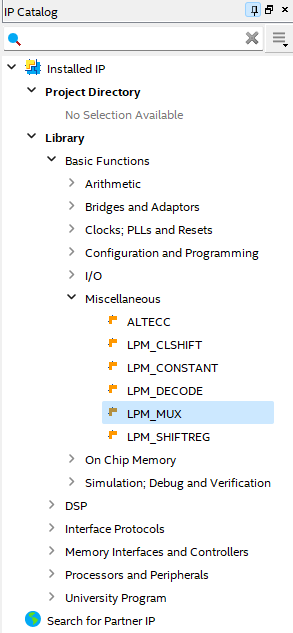
\includegraphics[scale=0.65]{IPCatalog1.png}
	\caption{Diagrama RTL del producto punto de dos vectores implementado en VHDL, sin inicializar la variable de suma de productos. \label{fig:ipcatalog1}}
\end{figure}

\begin{figure}[ht]
	\centering
	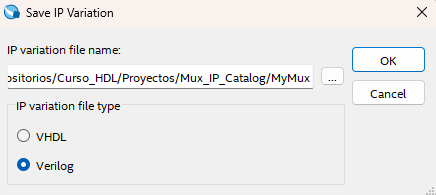
\includegraphics[scale=0.65]{IPCatalog2.png}
	\caption{Diagrama RTL del producto punto de dos vectores implementado en VHDL, sin inicializar la variable de suma de productos. \label{fig:ipcatalog2}}
\end{figure}

\begin{figure}[ht]
	\centering
	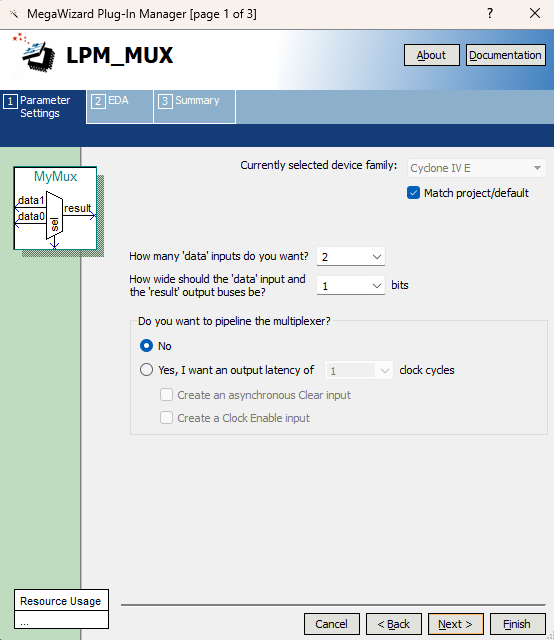
\includegraphics[scale=0.65]{IPCatalog3.png}
	\caption{Diagrama RTL del producto punto de dos vectores implementado en VHDL, sin inicializar la variable de suma de productos. \label{fig:ipcatalog3}}
\end{figure}

\begin{figure}[ht]
	\centering
	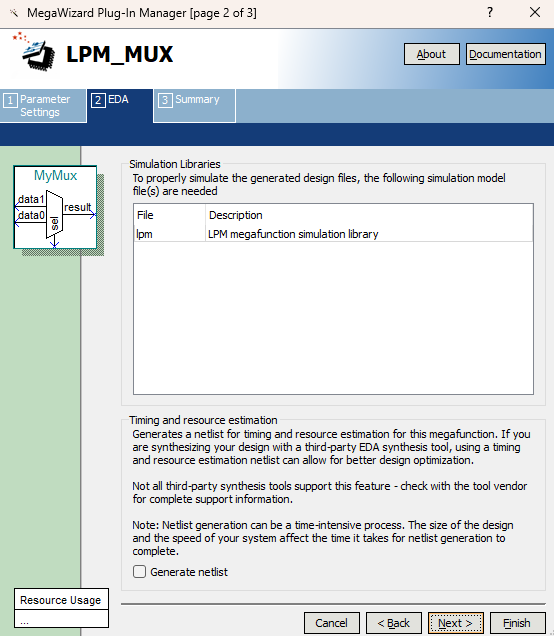
\includegraphics[scale=0.65]{IPCatalog4.png}
	\caption{Diagrama RTL del producto punto de dos vectores implementado en VHDL, sin inicializar la variable de suma de productos. \label{fig:ipcatalog4}}
\end{figure}

\begin{figure}[ht]
	\centering
	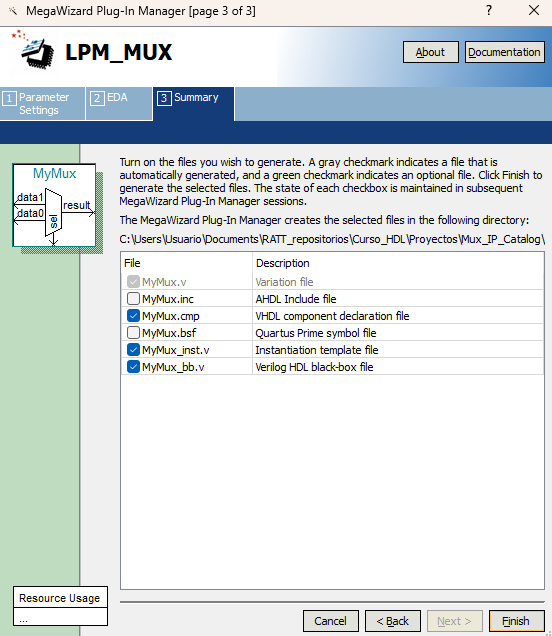
\includegraphics[scale=0.65]{IPCatalog5.png}
	\caption{Diagrama RTL del producto punto de dos vectores implementado en VHDL, sin inicializar la variable de suma de productos. \label{fig:ipcatalog5}}
\end{figure}

\begin{figure}[ht]
	\centering
	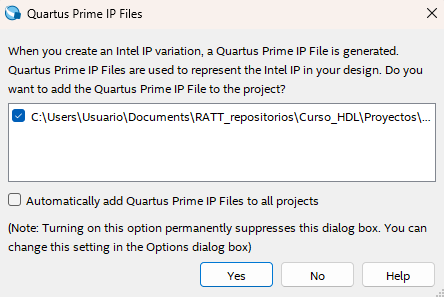
\includegraphics[scale=0.65]{IPCatalog6.png}
	\caption{Diagrama RTL del producto punto de dos vectores implementado en VHDL, sin inicializar la variable de suma de productos. \label{fig:ipcatalog6}}
\end{figure}

\begin{figure}[ht]
	\centering
	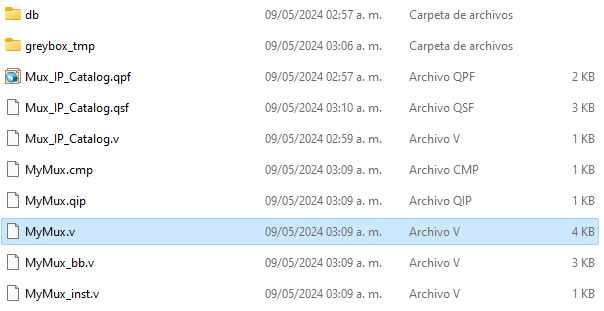
\includegraphics[scale=0.65]{IPCatalog7.png}
	\caption{Diagrama RTL del producto punto de dos vectores implementado en VHDL, sin inicializar la variable de suma de productos. \label{fig:ipcatalog7}}
\end{figure}

\begin{figure}[ht]
	\centering
	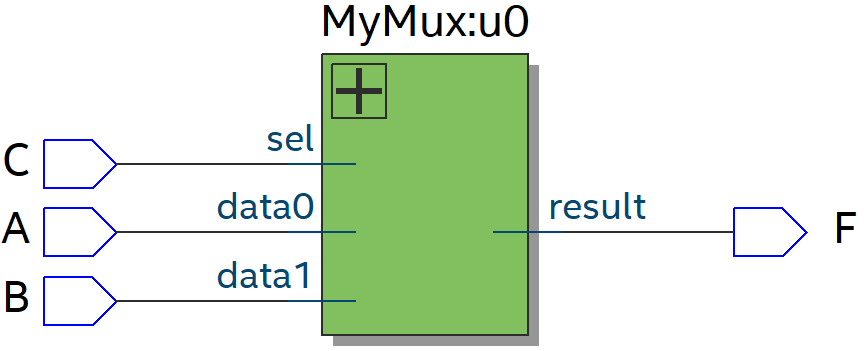
\includegraphics[scale=0.65]{Mux_IP_Catalog_RTL.png}
	\caption{Diagrama RTL del producto punto de dos vectores implementado en VHDL, sin inicializar la variable de suma de productos. \label{fig:mux_ipcatalog_rtl}}
\end{figure}

\begin{figure}[ht]
	\centering
	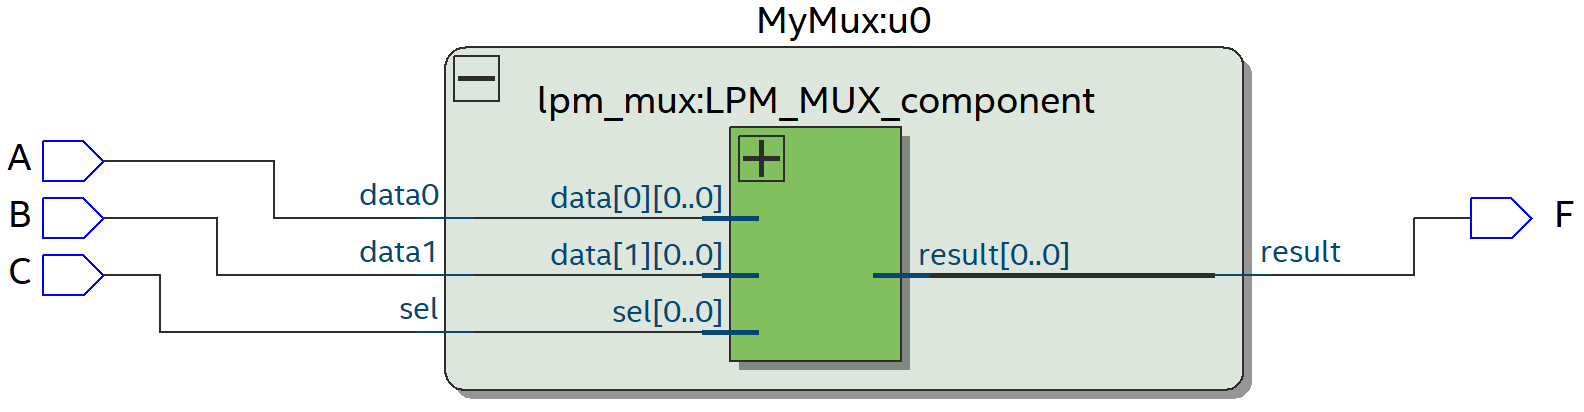
\includegraphics[scale=0.65]{Mux_IP_Catalog_RTL2.png}
	\caption{Diagrama RTL del producto punto de dos vectores implementado en VHDL, sin inicializar la variable de suma de productos. \label{fig:mux_ipcatalog_rtl2}}
\end{figure}

\begin{figure}[ht]
	\centering
	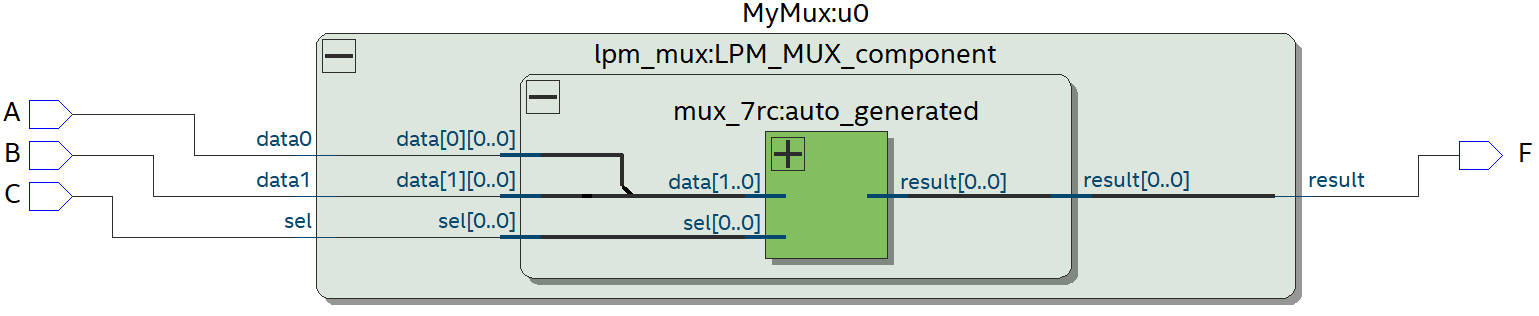
\includegraphics[scale=0.65]{Mux_IP_Catalog_RTL3.png}
	\caption{Diagrama RTL del producto punto de dos vectores implementado en VHDL, sin inicializar la variable de suma de productos. \label{fig:mux_ipcatalog_rtl3}}
\end{figure}

\begin{figure}[ht]
	\centering
	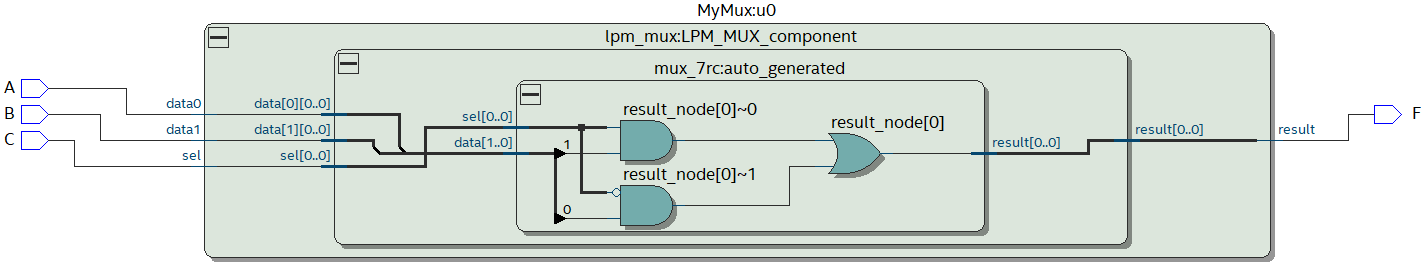
\includegraphics[scale=0.65]{Mux_IP_Catalog_RTL4.png}
	\caption{Diagrama RTL del producto punto de dos vectores implementado en VHDL, sin inicializar la variable de suma de productos. \label{fig:mux_ipcatalog_rtl4}}
\end{figure}

\begin{figure}[ht]
	\centering
	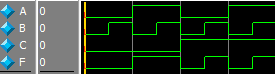
\includegraphics[scale=1.4]{Mux_IP_Catalog_Wave.png}
	\caption{Simulación del producto punto de dos vectores en VHDL, sin inicializar la variable de suma de productos, con el visor de formas de onda de ModelSim (base binaria). \label{fig:for_loop2_vhdl_wavebi}}
\end{figure}